\cleardoublepage
\chapter{The Protocol}
\label{protocol_chapter}

\newcommand{\Wconflict}{\text{\sc Conflict}\xspace}

\newcommand{\Obj}{{\sf Obj}}
\newcommand{\partitions}{\ensuremath{\mathsf{partitions}}}
\newcommand{\TxVars}{\ensuremath{\mathsf{TxVars}}}
\newcommand{\Tvar}{\ensuremath{\mathsf{T}}}
\newcommand{\Svar}{\ensuremath{\mathsf{S}}}
\newcommand{\Clients}{\ensuremath{\mathsf{Clients}}}
\newcommand{\Partitions}{\ensuremath{\mathsf{Partitions}}}
\newcommand{\VCSet}{\ensuremath{\mathsf{VerVector}}}
\newcommand{\VCType}{\ensuremath{\mathit{V}}}
\newcommand{\WSType}{\ensuremath{\mathit{WS}}}

\newcommand{\MsgLabel}{\ensuremath{\mathsf{MessageLabels}}}
\newcommand{\Messages}{\ensuremath{\mathsf{Messages}}}

\newcommand{\localWS}{\ensuremath{\mathit{WS}}}
\newcommand{\partitionOf}{\ensuremath{\mathsf{partition}}}
\newcommand{\WS}{\ensuremath{\mathsf{WS}}}
\newcommand{\WriteSets}{\ensuremath{\mathsf{WriteSets}}}

\newcommand{\Tx}{\ensuremath{\mathsf{Tx}}}
\newcommand{\VCdep}{\ensuremath{\mathsf{Vdep}}}
\newcommand{\VCaggr}{\ensuremath{\mathsf{Vsnap}}}
\newcommand{\Vaggr}{\ensuremath{\mathsf{Vaggr}}}
\newcommand{\Value}{\ensuremath{\mathsf{Value}}}
\newcommand{\CommitTime}{\ensuremath{\mathsf{CommitTime}}}
\newcommand{\Vcomm}{\ensuremath{\mathsf{Vcomm}}}

\newcommand{\Versions}{\ensuremath{\mathsf{Versions}}}
\newcommand{\pending}{\text{\sc pending}}
\newcommand{\ready}{\text{\sc decided}}
\newcommand{\CQentries}{\ensuremath{\mathsf{CQentries}}}
\newcommand{\CLogs}{\ensuremath{\mathsf{CLogs}}}
\newcommand{\VLogs}{\ensuremath{\mathsf{Vlogs}}}
\newcommand{\PState}{\ensuremath{\mathsf{PState}}}

\newcommand{\CommitLog}{\ensuremath{\mathsf{CommitLog}}}
\newcommand{\CommitQueue}{\ensuremath{\mathsf{CommitQueue}}}
\newcommand{\VersionLog}{\ensuremath{\mathsf{VersionLog}}}
\newcommand{\LastTransactionProcessed}{\ensuremath{\mathsf{LastPrep}}}
\newcommand{\LocalTime}{\ensuremath{\mathsf{Vtotal}}}
\newcommand{\LocalEntry}{\ensuremath{\mathit{MVC}}}
\newcommand{\hasRead}{\ensuremath{\mathsf{HasRead}}}

\newcommand{\VCzero}{\ensuremath{\mathbf{0}_V}}
\newcommand{\dom}{\ensuremath{\mathsf{dom}}}

\newcommand{\Cevent}{\ensuremath{\mathsf{ConcEvents}}}
\newcommand{\actionOf}{\ensuremath{\mathsf{ActionOf}}}
\newcommand{\Act}{\ensuremath{\mathsf{Act}}}
\newcommand{\actstart}{\ensuremath{\mathsf{start}}}
\newcommand{\actwrite}{\ensuremath{\mathsf{write}}}
\newcommand{\actread}{\ensuremath{\mathsf{read}}}
\newcommand{\actreadreturn}{\ensuremath{\mathsf{read}\_\mathsf{return}}}
\newcommand{\actabort}{\ensuremath{\mathsf{abort}}}
\newcommand{\actreadrequest}{\ensuremath{\mathsf{read}\_\mathsf{request}}}
\newcommand{\actwritetolog}{\ensuremath{\mathsf{writeToVlog}}}
\newcommand{\actcommit}{\ensuremath{\mathsf{commit}}}
\newcommand{\actcommitreturn}{\ensuremath{\mathsf{commit}\_\mathsf{return}}}
\newcommand{\actprepare}{\ensuremath{\mathsf{prepare}}}
\newcommand{\actdecide}{\ensuremath{\mathsf{decide}}}
\newcommand{\actupdate}{\ensuremath{\mathsf{update}}}

\newcommand{\TxNew}{\ensuremath{\mathsf{TxNew}}}
\newcommand{\TxWrite}{\ensuremath{\mathsf{TxWrite}}}
\newcommand{\TxFirstRead}{\ensuremath{\mathsf{TxFirstRead}}}
\newcommand{\TxOtherRead}{\ensuremath{\mathsf{TxOtherRead}}}
\newcommand{\TxReadAbort}{\ensuremath{\mathsf{TxReadAbort}}}
\newcommand{\TxReadSuccessful}{\ensuremath{\mathsf{TxReadSuccess}}}
\newcommand{\TxReadRequestOld}{\ensuremath{\mathsf{TxOldReadRequest}}}
\newcommand{\TxReadRequestNew}{\ensuremath{\mathsf{TxNewReadRequest}}}
\newcommand{\TxReadRequestAbort}{\ensuremath{\mathsf{TxAbortReadRequest}}}
\newcommand{\TxReadOnlyCommit}{\ensuremath{\mathsf{TxReadOnlyCommit}}}
\newcommand{\TxStartCommit}{\ensuremath{\mathsf{TxStartCommit}}}
\newcommand{\TxEndCommit}{\ensuremath{\mathsf{TxEndCommit}}}
\newcommand{\TxWriteConflictConcurrent}{\ensuremath{\mathsf{TxWWConfConcurrent}}}
\newcommand{\TxWriteConflictCommitted}{\ensuremath{\mathsf{TxWWConfCommitted}}}
\newcommand{\TxNoWriteConflict}{\ensuremath{\mathsf{TxNoWWConf}}}
\newcommand{\TxDecideTrue}{\ensuremath{\mathsf{TxDecideTrue}}}
\newcommand{\TxDecideFalse}{\ensuremath{\mathsf{TXDecideFalse}}}
\newcommand{\TxUpdate}{\ensuremath{\mathsf{TxUpdate}}}

\newcommand{\msgreadrequest}{\ensuremath{\mathsf{READREQUEST}}}
\newcommand{\msgreadreturn}{\ensuremath{\mathsf{READRETURN}}}
\newcommand{\msgprepare}{\ensuremath{\mathsf{PREPARE}}}
\newcommand{\msgdecide}{\ensuremath{\mathsf{DECIDE}}}
\newcommand{\msgvote}{\ensuremath{\mathsf{VOTE}}}

\newcommand{\lastCompatibleVersion}{\ensuremath{\mathsf{lastCompatible}}}
\newcommand{\fixSnapshot}{\ensuremath{\mathsf{fixSnapshot}}}
\newcommand{\updateCommitVC}{\ensuremath{\mathsf{CommitVC}}}

\newcommand{\CommitVector}{\ensuremath{\mathsf{CommitVC}}}

\newcommand{\abort}{\text{\sc abort}}
\newcommand{\commit}{\text{\sc commit}}

\newcommand{\access}{\ensuremath{\mathsf{Access}}}

\newcommand{\TO}{\ensuremath{\mathsf{to}}}

\newcommand{\startEvent}{\ensuremath{\mathsf{startEvent}}}

\newcommand{\readmessages}{\ensuremath{\mathsf{readMessages}}}
\newcommand{\commitmessages}{\ensuremath{\mathsf{commitMessages}}}
\newcommand{\updatemessages}{\ensuremath{\mathsf{updateMessages}}}

\newcommand{\vlsubseteq}{\ensuremath{\sqsubseteq_{\mathsf{VL}}}}
\newcommand{\dvsubseteq}{\ensuremath{\sqsubseteq_{\mathsf{VC}}}}

\newcommand{\lastVC}{\ensuremath{\mathsf{lastVC}}}

\newcommand{\at}{\ensuremath{@}}

\newcommand{\localVaggr}{\mathit{Vaggr}}
\newcommand{\localVdep}{\mathit{Vdep}}
\newcommand{\argVCaggr}{\ensuremath{\mathit{Vsnap}}}
\newcommand{\argVCdep}{\ensuremath{\mathit{Vdep}}}
\newcommand{\argHasRead}{\mathit{HasRead}}
\newcommand{\maxVC}{\ensuremath{\mathit{MaxVC}}}
\newcommand{\argMaxVC}{\ensuremath{\mathit{MaxVC}}}
\newcommand{\argVLog}{\ensuremath{\mathit{VersionLog}}}

\newcommand{\READREQUEST}{{\tt READREQUEST}}
\newcommand{\READRETURN}{{\tt READRETURN}}
\newcommand{\PREPARE}{{\tt PREPARE}}
\newcommand{\DECIDE}{{\tt DECIDE}}
\newcommand{\VOTE}{{\tt VOTE}}
\newcommand{\ABORT}{{\tt ABORT}}

\newcommand{\outcome}{\mathit{decision}}
\newcommand{\false}{\bottom}
\newcommand{\true}{\top}

\newcommand{\cqueue}{\CommitQueue}
\newcommand{\cqhead}{\CommitQueue.{\sf head}}
\newcommand{\cqupdate}{\CommitQueue.{\sf update}}
\newcommand{\cqremove}{\CommitQueue.{\sf remove}}
\newcommand{\cqput}{\CommitQueue.{\sf put}}

\newcommand{\cladd}{\CommitLog.{\sf add}}

\newcommand{\vlapply}{\VersionLog.{\sf add}}
\newcommand{\vllast}{\VersionLog.{\sf last}}
\newcommand{\last}{{\rm last}}
\newcommand{\ver}{\mathit{ver}}

\newcommand{\mrvc}{\LocalTime}

\newcommand{\lastprep}{\LastTransactionProcessed}

\newcommand{\parti}{\mathit{p_i}}
\newcommand{\partj}{\mathit{s_j}}

\newcommand{\transtype}{{\sf Tx}}
\newcommand{\keytype}{{\sf Object}}
\newcommand{\valuetype}{{\sf Value}}
\newcommand{\vctype}{{\sf VerVector}}

\newcommand{\val}{{\sf val}}

\newcommand{\tx}{\ensuremath{\mathit{T}}}

\newcommand{\commitVC}{\mathit{Vcomm}}

\newcommand{\localkey}{{\sf k}}
\newcommand{\localval}{{\sf v}}
\newcommand{\partitionof}{{\sf partition}}

\SetKwBlock{SubAlgoBlock}{}{end}
\newcommand{\SubAlgo}[2]{#1 \SubAlgoBlock{#2}}

\SetKw{Upon}{upon}
\SetKw{WhenReceived}{when received}
\SetKw{Send}{send}
\SetKw{Receive}{wait receive}
\SetKw{Until}{wait until}
\SetKw{KwFrom}{from}
\SetKw{KwTo}{to}
\SetKw{Throw}{throw}
\SetKw{Fun}{function}
\SetKw{Break}{break}
\SetKw{New}{new}

\todo{
Add an ``overview'' section with a figure that explains the protocol at a high level, step by step. We can do it as an example, denoting the messages between client and server. We can also say how the state (assuming an initial one) evolves with each step.

Another option is to use this figure in two places. In overview, the figure will explain the messages and steps. In the detailed section, use the figure as a running example.

Tradeoff of 2pc vs Ardekani et. al. atomic multicast (the difference with NMSI)

Design tradeoffs?
}

In this chapter, we describe how our protocol \todo{name} works. First, we present an overview of how the different participants interact. We follow with a formal description of the system model, and a description of the different data structures it encompasses. Next, we show how the protocol is implemented by going over the execution of a transaction.

\section{Overview}

Our protocol consists of three components: \emph{client} and \emph{server} processes that provide the system interface for managing transactions and its individual operations, respectively; and \emph{partitions}, managed by a server, and which manage individual data objects. Figure~\ref{fig:execution} shows an overview of an example execution of the protocol.

\subparagraph{Clients.} They provide the transactional interface of our protocol, namely \texttt{start}, \texttt{read}, \texttt{write} and \texttt{commit}. Our protocol uses optimistic concurrency control, and therefore the \texttt{start} and \texttt{write} operations are local to the client. \texttt{Read} operations are issued to servers, which in turn communicate with its partitions and return the values and metadata associated with the objects the client requested. At \texttt{commit} time, the client acts a coordinator of a \emph{two-phase commit protocol (2PC)} among all the participating servers, issuing \texttt{prepare} and \texttt{decide} operations. The written values buffered locally are transmitted to the servers at \texttt{prepare} time, together with the accumulated metadata for the objects that the client read. The decision to commit or abort a transaction is taken based on this metadata.

\subparagraph{Servers.} These processes handle three operations issued by clients: \texttt{read}, \texttt{prepare} and \texttt{decide}. For \texttt{reads}, it forwards the request to the partition responsible for the object being read. When receiving a \texttt{prepare} request for a certain transaction, the server checks for conflicts among concurrent transactions stored in a FIFO queue of transactions to be decided. If the transaction contained in the request does not conflict, it is added to the queue, and the server replies to the client with a positive vote. If the transaction is found to be conflicting, a negative vote is sent instead.

\subparagraph{Partitions.} A partition is responsible for fulfilling read requests on behalf of servers. Each partition contains non-overlapping sets of objects, storing them as a list of versions, in accordance with a multi-version concurrency control protocol. When executing a read request, a partition finds the appropriate version of the object being read in its state, and returns the object value, along with some metadata of the chosen version.

\begin{figure}[t]
\vspace{-2cm}
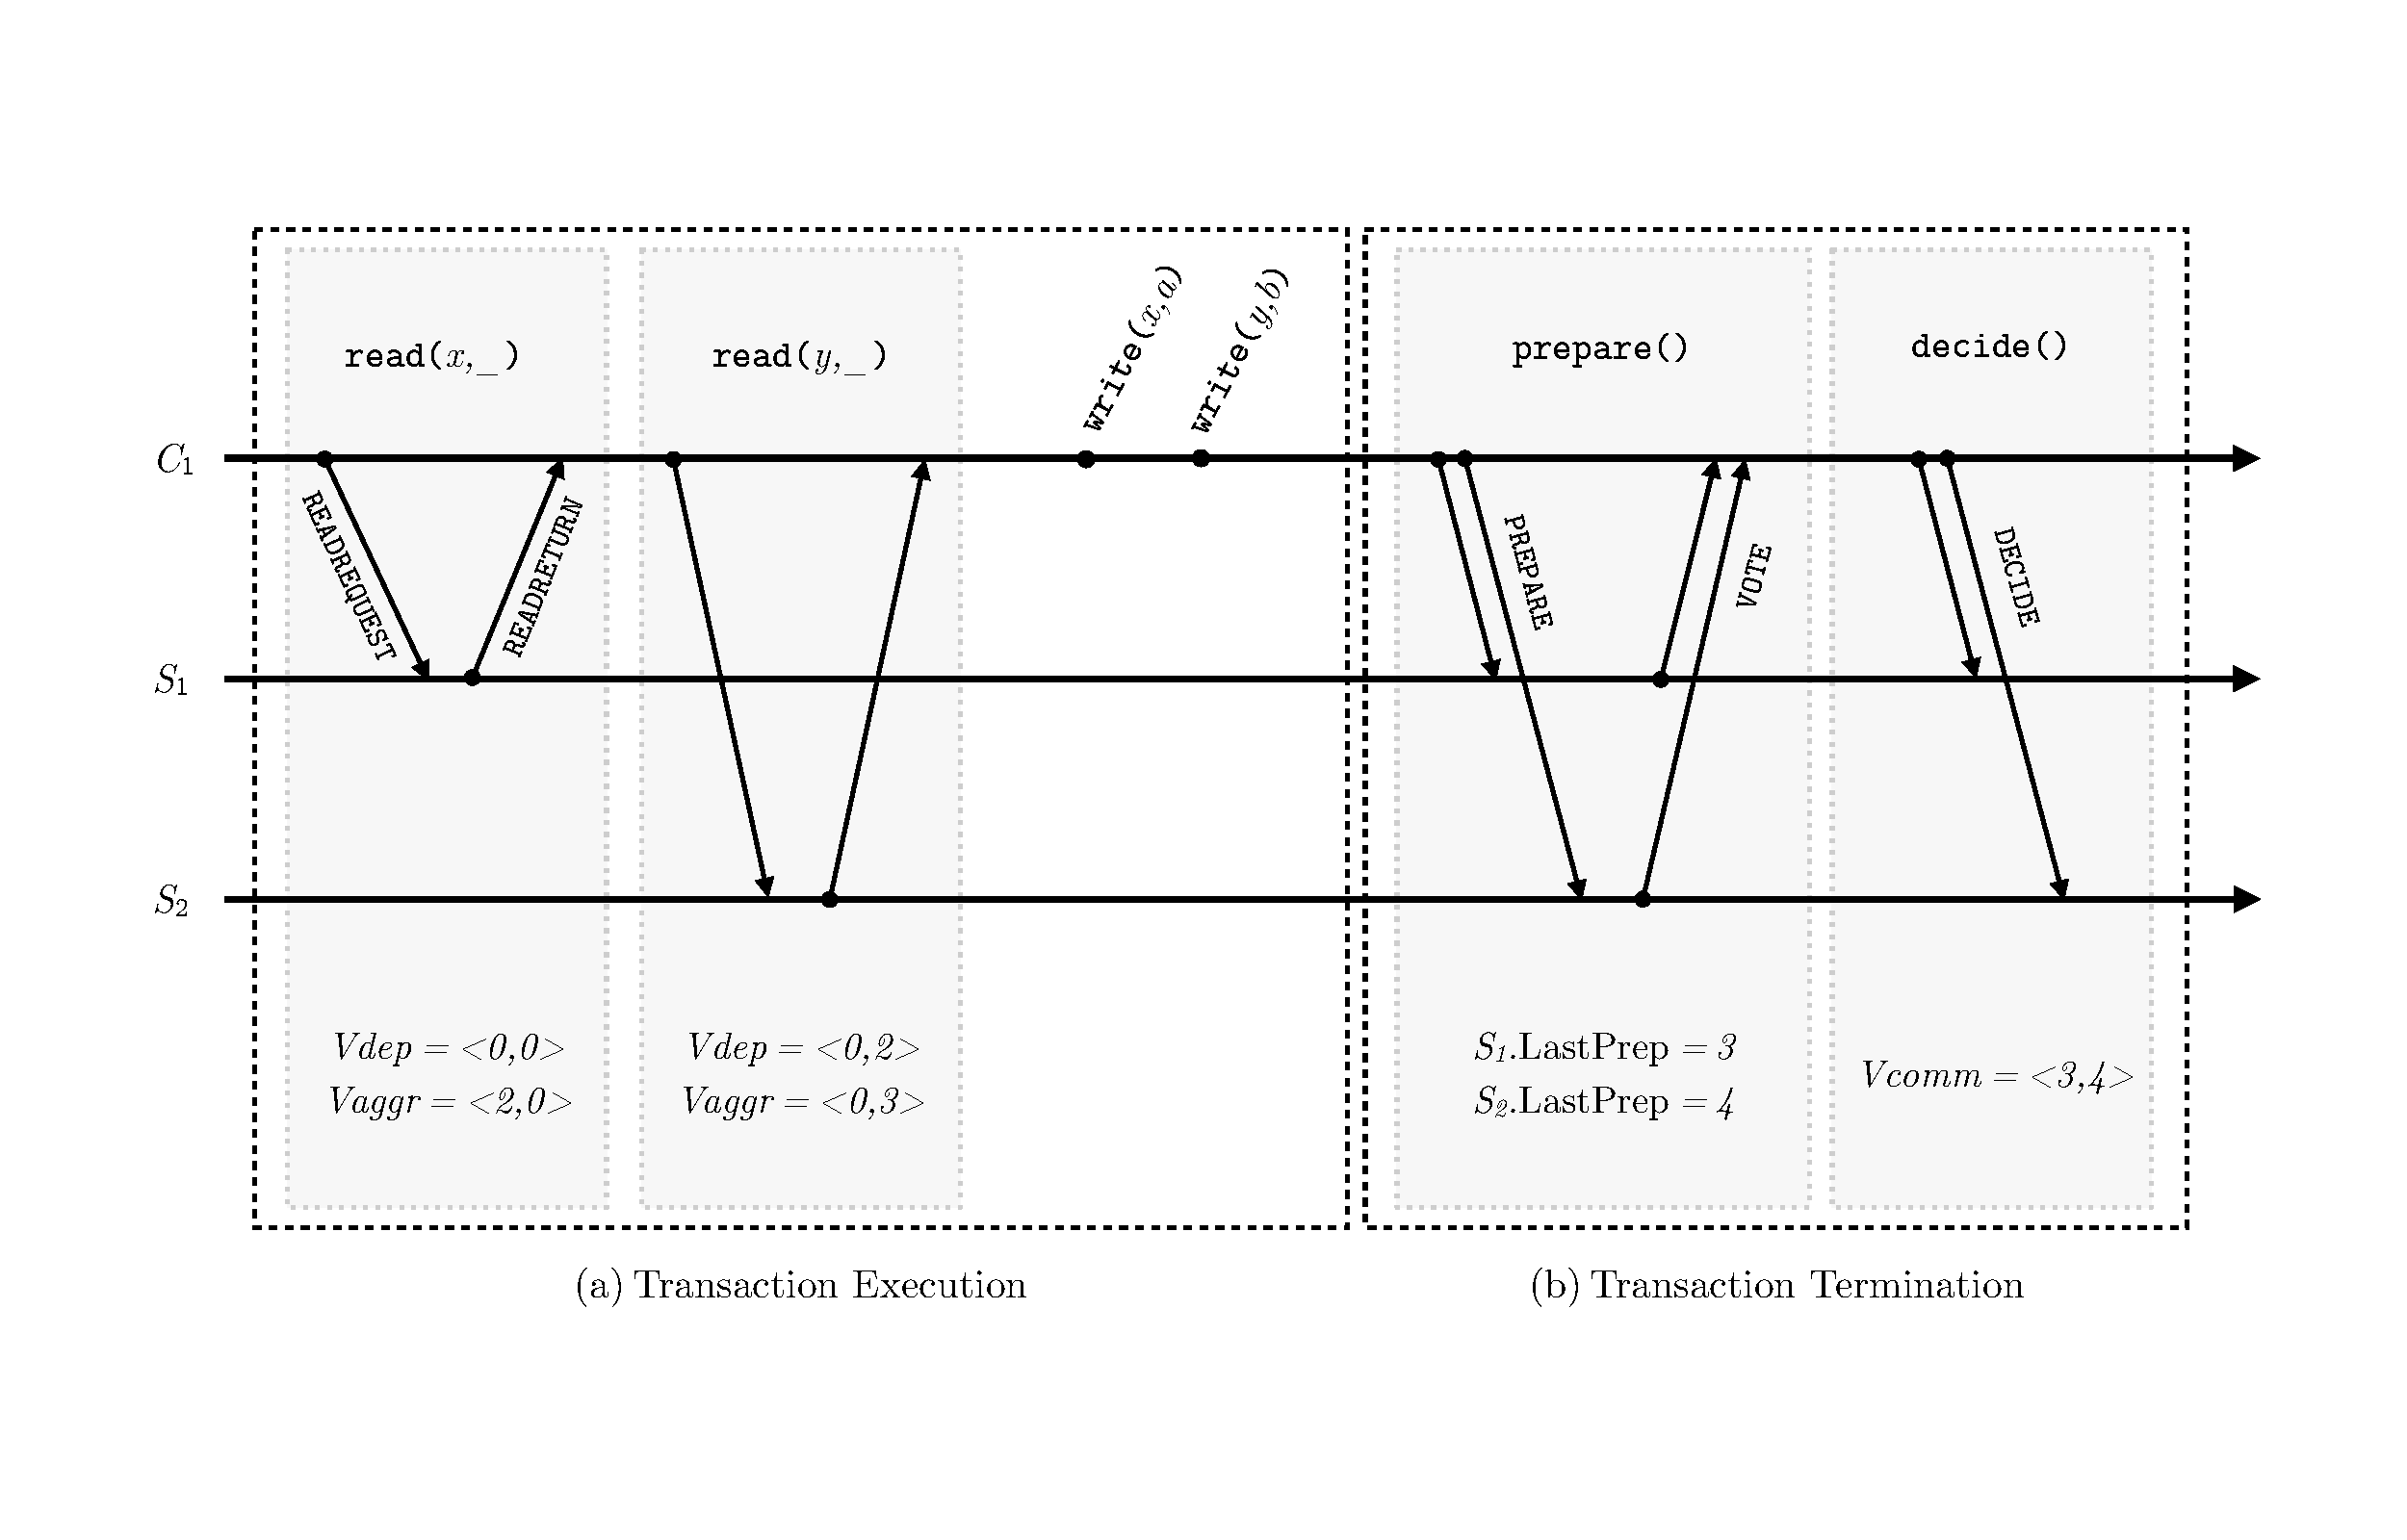
\includegraphics[width=\textwidth]{figures/ch4_execution.pdf}
\vspace{-2cm}
\caption{Message flow diagram of a sample execution, with message arrows labeled with their names in the protocol. The different interactions between a client and servers are shown in the shadowed regions. The operation performed by the client is shown at the top, and the state observed by the client at the end of each message exchange is summarised at the bottom.}
\label{fig:execution}
\end{figure}

\section{System Model}

\todo{Figure out how to fit this with the previous section}

We consider an asynchronous, message-passing system consisting of a set of reliable processes connected by reliable channels. Fault-tolerance concerns are orthogonal to the problem we address. The processes are split into two sets; a set of \emph{servers} $\mathcal{S} = \{s_1, \dots, s_N\}$, and a set of \emph{clients} $\mathcal{C} = \{c_1, \dots, c_M\}$. The system manages a set of objects $\Obj$ split into $N$ partitions, each stored by a server process. We let $\partitionOf(x)$ be the index of the partition the object $x$ belongs to, so that it is managed by server $s_{\partitionOf(x)}$. Clients execute transactions by communicating with servers. Transactions can be \emph{interactive}, i.e., when a transaction starts, the client does not know which operations it will perform in advance. Clients refer to transactions by their identifier from a set $\transtype$.

\section{Server data structures}

\todo{Data structures and protocol explanations are too tied together. Perhaps add an ``overview'' section before (of the protocol) so we can explain the structures without mixing the two.}

\todo{Look into \textsection 4.2 in GMU paper for a possible way to write this section.}

The data structures maintained by the protocol at a process are summarised in Figure~\ref{fig:prot-ds-table}. Each server $s_i$ maintains a counter $\lastprep$ of the number of update transactions that initiated their commit phase at the server. When such a transaction commits at a server $s_i$, it will be assigned a \emph{sequence number} $k$ derived from this counter. All the update operations by the transaction at $s_i$ are identified by a pair $(s_i, k)$, which we call dot~\citep{carlos-causality}. We call the order of transactions imposed by their sequence numbers issued by $s_i$ the \emph{commit order} at $s_i$.

% \begin{itemize}
%   \item $\lastprep$, a counter of the number of update transactions that initiated their commit phase at $s_i$. When a transaction commits at $s_i$, it will be assigned a \emph{sequence number} $k$ derived from this counter.
% \end{itemize}

\todo{Maybe move this to preliminaries? We have to justify doing PSI with VCs instead of NMSI's approach with dependence vectors}

To track the happens-before \todo{HB should be defined previously} relationship between transactions, we use \emph{version vectors}~\citep{version-vectors}. Such a vector consists of $N$ entries, one for each server, storing a non-negative integer. A version vector $V$ represents the set of dots $\{(s_i, k) \mid k \le V[i]\}$, which identify the writes by transactions whose sequence number at a server $s_i$ is no higher than $V[i]$. Version vectors are compared according to the following relation, showing when one vector covers more dots than another: $V_1 \sqsubseteq V_2 \iff \forall i.\ V_1[i] \le V_2[i]$. In addition, there exists a \emph{join} operation on vectors, taking their component-wise maximum. We we will denote this operation by $\max$ from now on. We also denote the set of all version vectors by $\VCSet$, and the vector with all entries set to $0$ by $\vec{0}$.

The protocol associates each committed transaction $\tx$ with a \emph{commit vector}---a version vector $V$ representing the dots that cover all the writes by $\tx$ as well as the writes of transactions preceding $\tx$ under happens-before \todo{HB}. In particular, the entry $V[i]$ for a server $s_i$ where $\tx$ wrote an object stores the sequence number of $\tx$ issued by $s_i$. A server $s_i$ maintains a list of update transactions that committed at the server in a $\CommitLog$, storing triples $\langle T,V_c,V_a\rangle$. Here, $\tx$ is the identifier of a committed transaction, and $V_c$ is its commit vector. The $\CommitLog$ at $s_i$ is totally ordered according to the value $V_c[i]$, which follows the commit order at $s_i$. The last component of the triple, $V_a$, represents the join of the commit vectors of all the transactions up to $\tx$ in $\CommitLog$. This \emph{aggregate} vector is stored for efficiency---the server also caches the aggregate vector of the last committed transaction in a variable $\LocalTime$. Initially, the $\CommitLog$ contains a single dummy entry $\langle \_, \vec{0}, \vec{0} \rangle$.

\todo{Note how the order of T's and the order of versions relates, like in \textsection 5.1 of Blotter}

A server $s_i$ maintains multiple versions of the objects it manages, stored in a mapping $\VersionLog$, which we call the \emph{database}. This log maps an object to a a list of \emph{versions}, pairs of a value and the commit vector of the transaction that wrote this value. The $\VersionLog$ is ordered by the $i$-th component of the commit vector of each version, which follows the commit order of transactions at $s_i$. We denote by $\VersionLog[x].\last$ the most recent entry in the list for the object $x$.

Finally, a server $s_i$ maintains an ordered queue $\CommitQueue$ of transactions trying to commit updates at the server. The queue has entries of two types. An entry $\langle \pending, T, \localWS \rangle$ means that $\tx$ is successfully prepared to commit at $s_i$, but the final decision on it is not yet known; $\localWS$ is the \emph{write-set} of the transaction, containing object-value pairs. An entry $\langle \ready, T, \localWS, V \rangle$ in the queue means that $\tx$ has been decided to commit with a commit vector $V$, but its writes have not yet been added to the $\VersionLog$. The order of transactions in $\CommitQueue$ follows the commit order at the server.

\begin{figure}[t]
\noindent\adjustbox{max width=\paperwidth}{\footnotesize
\begin{tabularx}{\linewidth}{|c|p{5.5cm}|X|}
  \hline
  \multicolumn{3}{|c|}{\textbf{Variables at a server $s_i$}}\\
  \hline
  $\lastprep$ & {\sf Integer} & The number of update transactions that tried to
  commit at the server.
\\
  \hline
  $\CommitLog$
  & ${\sf Sequence}[\langle\transtype\ {\sf T},$ $\vctype\ \Vcomm, \vctype\ \Vaggr \rangle]$
  & Log of update transactions $T$ committed at the server, ordered by
  $V_c[i]$. Here $V_c$ is the commit vector of $T$ and $V_a$ is the aggregate
  vector of $T$: the join of the commit vectors of all transactions up to $T$ in
  $\CommitLog$.
\\
  \hline
  $\LocalTime$ & $\vctype$ & The join of the commit vectors of all
  transactions in $\CommitLog$.
\\
  \hline
  $\VersionLog$ & ${\sf Map}[\keytype,$ ${\sf
    Set}[\langle \valuetype\ \val, \vctype\ \Vcomm\rangle]]$ & Database:
  a mapping from objects to lists of pairs of a value and the
  commit vector of the transaction that wrote it. The lists are ordered
  by the $i$-th component of the commit vectors.
\\
\hline
  $\CommitQueue$ & ${\sf Sequence}[\langle \transtype, \pending, {\sf WriteSet} \rangle \cup
  \langle \transtype, \ready, {\sf WriteSet}, \vctype\rangle]$ &
  Queue containing information about update transactions trying to commit
  at the server.
\\
  \hline
  \multicolumn{3}{|c|}{\textbf{Context for a transaction $T$ at a client $c_i$}} \\
  \hline
  $T.\WS$ & ${\sf WriteSet}$ & Write-set of $T$.
\\
  \hline
  $T.\hasRead$ & ${\sf Vector}[{\sf Bool}]$ & Mapping showing whether $T$  has
  read a given partition.
\\
  \hline
  $T.\VCaggr$ & $\vctype$ & Snapshot vector: determines snapshots fixed at
  partitions $T$ has read from and possible causal dependencies at all other
  partitions.
  \\
  \hline
  $T.\VCdep$ & $\vctype$ & Dependency vector, representing all causal
  dependencies developed by $T$ during its execution.
\\
  \hline
\end{tabularx}
}
\caption{List of variables used in the protocol, where
  ${\sf WriteSet} = {\sf Set}[\langle \keytype, \valuetype \rangle]$. The orders
  of entries in $\CommitLog$, $\VersionLog$ and $\CommitQueue$ are consistent
  with the commit order of transactions the entries are associated with. We
  select the components of various tuples using the names given in the figure. \todo{Fix table, weird spacing in middle column}}
\label{fig:prot-ds-table}
\end{figure}

\section{Protocol Description}

\todo{
  \begin{itemize}
    \item Revisit captions for pseudocode figures
    \item Think if \emph{causal dependency} is already defined in a previous section
    \item Mention that we disallow blind updates
  \end{itemize}
}

\subsection{Transaction Execution}

\begin{figure}[h]
\begin{algorithm}[H]
  \setcounter{AlgoLine}{0}
  \SubAlgo{\Fun ${\tt start}()$\label{alg:start_tx_start}}{
    \Return{$\KwSty{new}\ \transtype(\WS= \emptyset, \hasRead =
      \vec{\bot}, \VCaggr = \vec{0}, \VCdep =
      \vec{0})$};\label{alg:start_tx_end}}

  \smallskip

  \SubAlgo{\Fun ${\tt write}(T, x, v)$\label{alg:write_start}}{
    $\tx.\WS \leftarrow \left(\tx.\WS\ \backslash\ \{\langle x, \_ \rangle\}\right) \cup \{\langle x,v\rangle\}$\;\label{alg:write_end}
  }
\end{algorithm}
\caption{Initialisation of a transaction and update of an object \emph{x} at client $c_i$}
\end{figure}

A client executing a transaction $\tx$ maintains a transaction \emph{context} including several pieces of data, summarised in Figure~\ref{fig:prot-ds-table} and explained below. This context is initialised by the client when it starts a transaction (line~\ref{alg:start_tx_start}).

Since our protocol uses optimistic concurrency control, the execution of $\tx$ is speculative: clients read objects from servers and buffer writes locally. At the end of the execution, the decision whether to commit or abort a transaction is taken based on the existence of conflicts with concurrently executing transactions. When a transaction $\tx$ writes a value $v$ to an object $x$ (line~\ref{alg:write_start}), the client buffers this write in $\tx$'s \emph{write-set}, $\tx.\WS$, while discarding any previously written value of $x$.

When the transaction $\tx$ issues a read operation on an object $x$ (line~\ref{alg:read_start}), the client will first check $\tx.\WS$ (line~\ref{alg:read_ws_check}): if $\tx$ has already written to $x$, the value stored in the write-set is returned. Otherwise, and assuming that $j = \partitionOf(x)$, the client sends a $\READREQUEST$ message to the server $s_j$ to fetch the value of the object (line~\ref{alg:read_send}).

When the transaction $\tx$ reads an object from a partition $j$ for the first time, the server $s_j$ fixes a \emph{snapshot} of versions from which it will serve all future reads by $\tx$. This snapshot is defined by an integer $k$: it will include the versions written by all the transactions that committed at the server with a sequence number up to $k$. The client keeps this information in the transaction context, by storing $k$ in the $j$-th entry of a \emph{snapshot vector} $\tx.\VCaggr$, and by marking the current partition as read in $\tx.\hasRead$, a Boolean mapping its $j$-th entry to $\top$ if $\tx$ read an object from $j$, and $\bot$ otherwise. If $\tx.\hasRead[j]=\top$, then the vector $\tx.\VCaggr$ is equal to the join of the commit vectors of all transactions that at partition $j$ have a sequence number no higher than $\VCaggr[j]$, and vice versa.

\begin{figure}[h]
\begin{algorithm}[H]
  \SubAlgo{\Fun ${\tt read}(T, x)$\label{alg:read_start}}{
    \If{$\langle x, v \rangle \in \tx.\WS$\label{alg:read_ws_check}}{
      \Return{$v$}\;
    }

    $j \leftarrow \partitionof(x)$\;
    \Send{$\READREQUEST(x, T.\VCaggr, T.\hasRead)$} \KwTo $s_j$\;\label{alg:read_send}
    \Receive{$\READRETURN(m)$} \KwFrom $s_j$\;\label{alg:read_recv}
    \uIf{$m = \abort$} {
      \Throw{$\abort$}\;\label{alg:read_abort}
    }
    \ElseIf{$m = \langle v,\localVdep,\localVaggr \rangle$\label{alg:read_msg_decomp}}{
      $\tx.\hasRead[j] \leftarrow \true$\;
      $\tx.\VCdep \leftarrow \max(\tx.\VCdep,\localVdep)$\;\label{alg:read_upd_vcdep}
      $\tx.\VCaggr \leftarrow \max(\tx.\VCaggr,\localVaggr)$\;\label{alg:read_upd_vcaggr}
      \Return{$v$}\;\label{alg:read_end}
    }
  }
  \smallskip
  \SubAlgo{\WhenReceived $\READREQUEST(x, \argVCaggr, \argHasRead)$ \KwFrom $c_j$\label{alg:read_req_start}}{
    \uIf{$\argHasRead[i]$\label{alg:read_req_read_check}} {
      $V \leftarrow \argVCaggr$\;\label{alg:read_req_read_maxvc}
    }
    \Else{\label{alg:read_req_read_check_else}
      \Until{$\mrvc[i] \ge \argVCaggr[i]$}\;\label{alg:read_req_wait}
      $r \leftarrow \max\{r \in \CommitLog \mid \forall j.\, \argHasRead[j] {\implies} \left(r.\Vaggr[j] \le \argVCaggr[j]\right)\}$\;\label{alg:max_vc_search}
      \If{$r.\Vaggr[i] < \argVCaggr[i]$\label{alg:read_req_abort_check}}{
        \Send{$\READRETURN(\abort)$} \KwTo $c_j$\;\label{alg:read_req_abort}
        \Return\;
      }
      $V \leftarrow r.\Vaggr$\;\label{alg:read_req_unread_maxvc}
    }
    $\ver = \max\{\ver \in \VersionLog \mid ver.\Vcomm[i] \le V[i]\}$\; \label{alg:chose-version}
    \Send{$\READRETURN(\ver.\val, \ver.\Vcomm,V)$} \KwTo $c_j$\;\label{alg:read_req_end}
  }
\end{algorithm}
\caption{Local and remote read of object \emph{x}}
\end{figure}

\todo{First mention of causal dependency} Thus, the entries of the snapshot vector for partitions that $\tx$ has not yet read from delimit all the possible causal dependencies $\tx$ may develop at these partitions if it keeps reading objects from the snapshots it has already fixed.

Both $\tx.\VCaggr$ and $\tx.\hasRead$ are supplied by the client when issuing a read operation on object $x$, by using them as parameters to the $\READREQUEST$ message sent to a server $s_i$. When the server receives this message (line~\ref{alg:read_req_start}), it first checks, using the $\hasRead$ mapping, if the transaction has read from it before (line~\ref{alg:read_req_read_check}). In this case, the snapshot is determined by $\VCaggr[i]$, and the server returns the latest version $\mathit{ver}$ of the object $x$ written by a transaction in the snapshot, i.e., with a sequence number no higher than $\VCaggr[i]$ (line~\ref{alg:chose-version}). This version is determined by examining the $i$-th entry of the commit vectors in $\VersionLog$. The server then replies to the client with a $\READRETURN$ message containing the value of the chosen version and its associated version vector, as well as the unmodified snapshot vector provided by the client: since the server used a previously fixed snapshot, no updates to the vector are required.

% \begin{figure}[t]
% 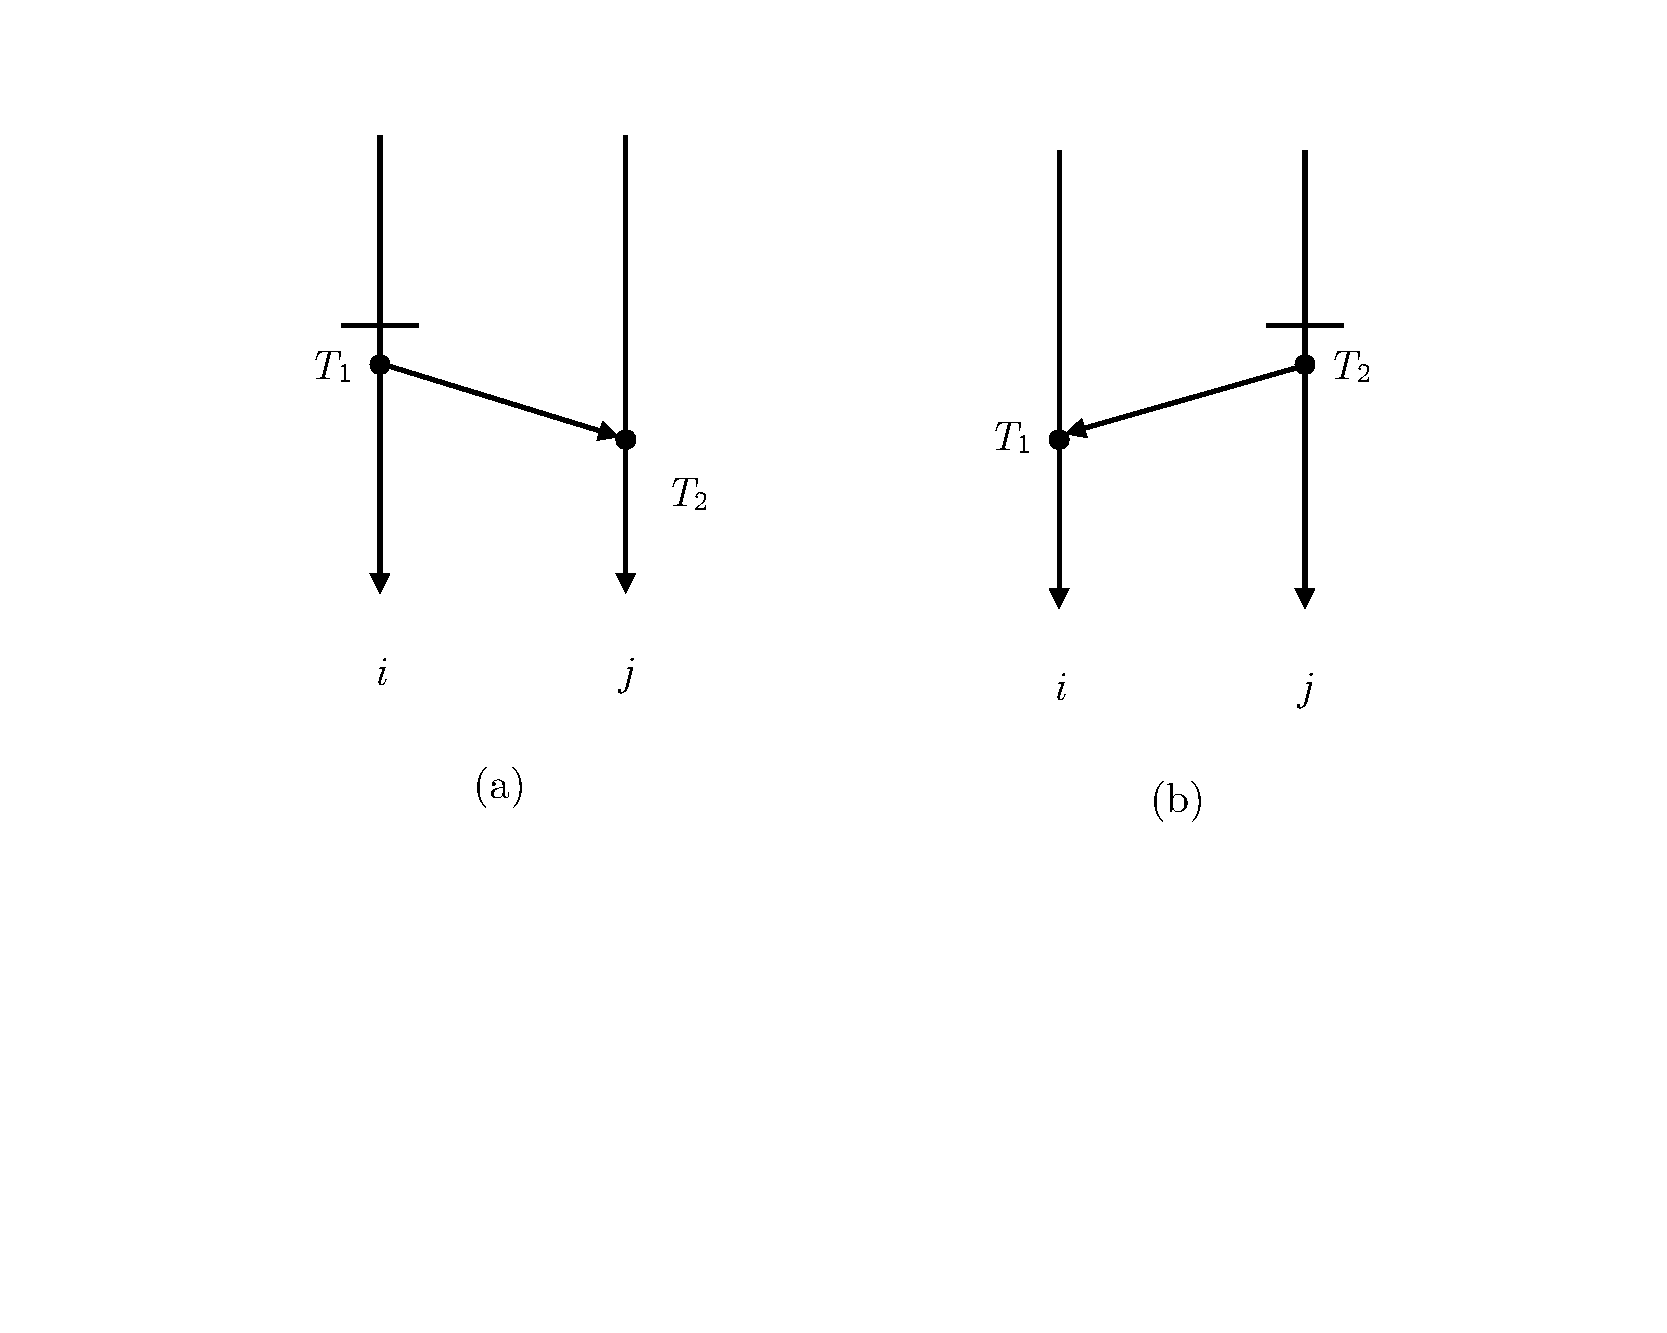
\includegraphics[width=\textwidth]{figures/ch4_snapshot_fork.pdf}
% \vspace{-5.5cm}
% \caption{Illustrations of the snapshot computation. Vertical lines depict the
%   commit order at the corresponding partitions (top to bottom) and horizontal
%   lines the cut-offs of various snapshots. Arrows between partitions depict
%   causal dependencies.}
% \label{fig:fig:snapshot_fork}
% \end{figure}

We now consider the case when the client is reading from the server $s_i$ for the first time (line~\ref{alg:read_req_read_check_else}), in which case, we have to fix the snapshot for the transaction $\tx$ at this server. Choosing a suitable snapshot is complicated by the fact that we allow transactions to be interactive---that is, we do not know in advance which objects will read in the future. We hence fix the snapshot in such a way that \emph{any} later read from this snapshot will be \emph{causally consistent} \todo{check usage, define in chapter 2 or 3} with any reads (past or future) from the snapshots that $\tx$ has already read, as specified by $\hasRead$ and $\VCaggr$. To ensure this, the snapshot we select has to satisfy two requirements.

\begin{figure}[t]
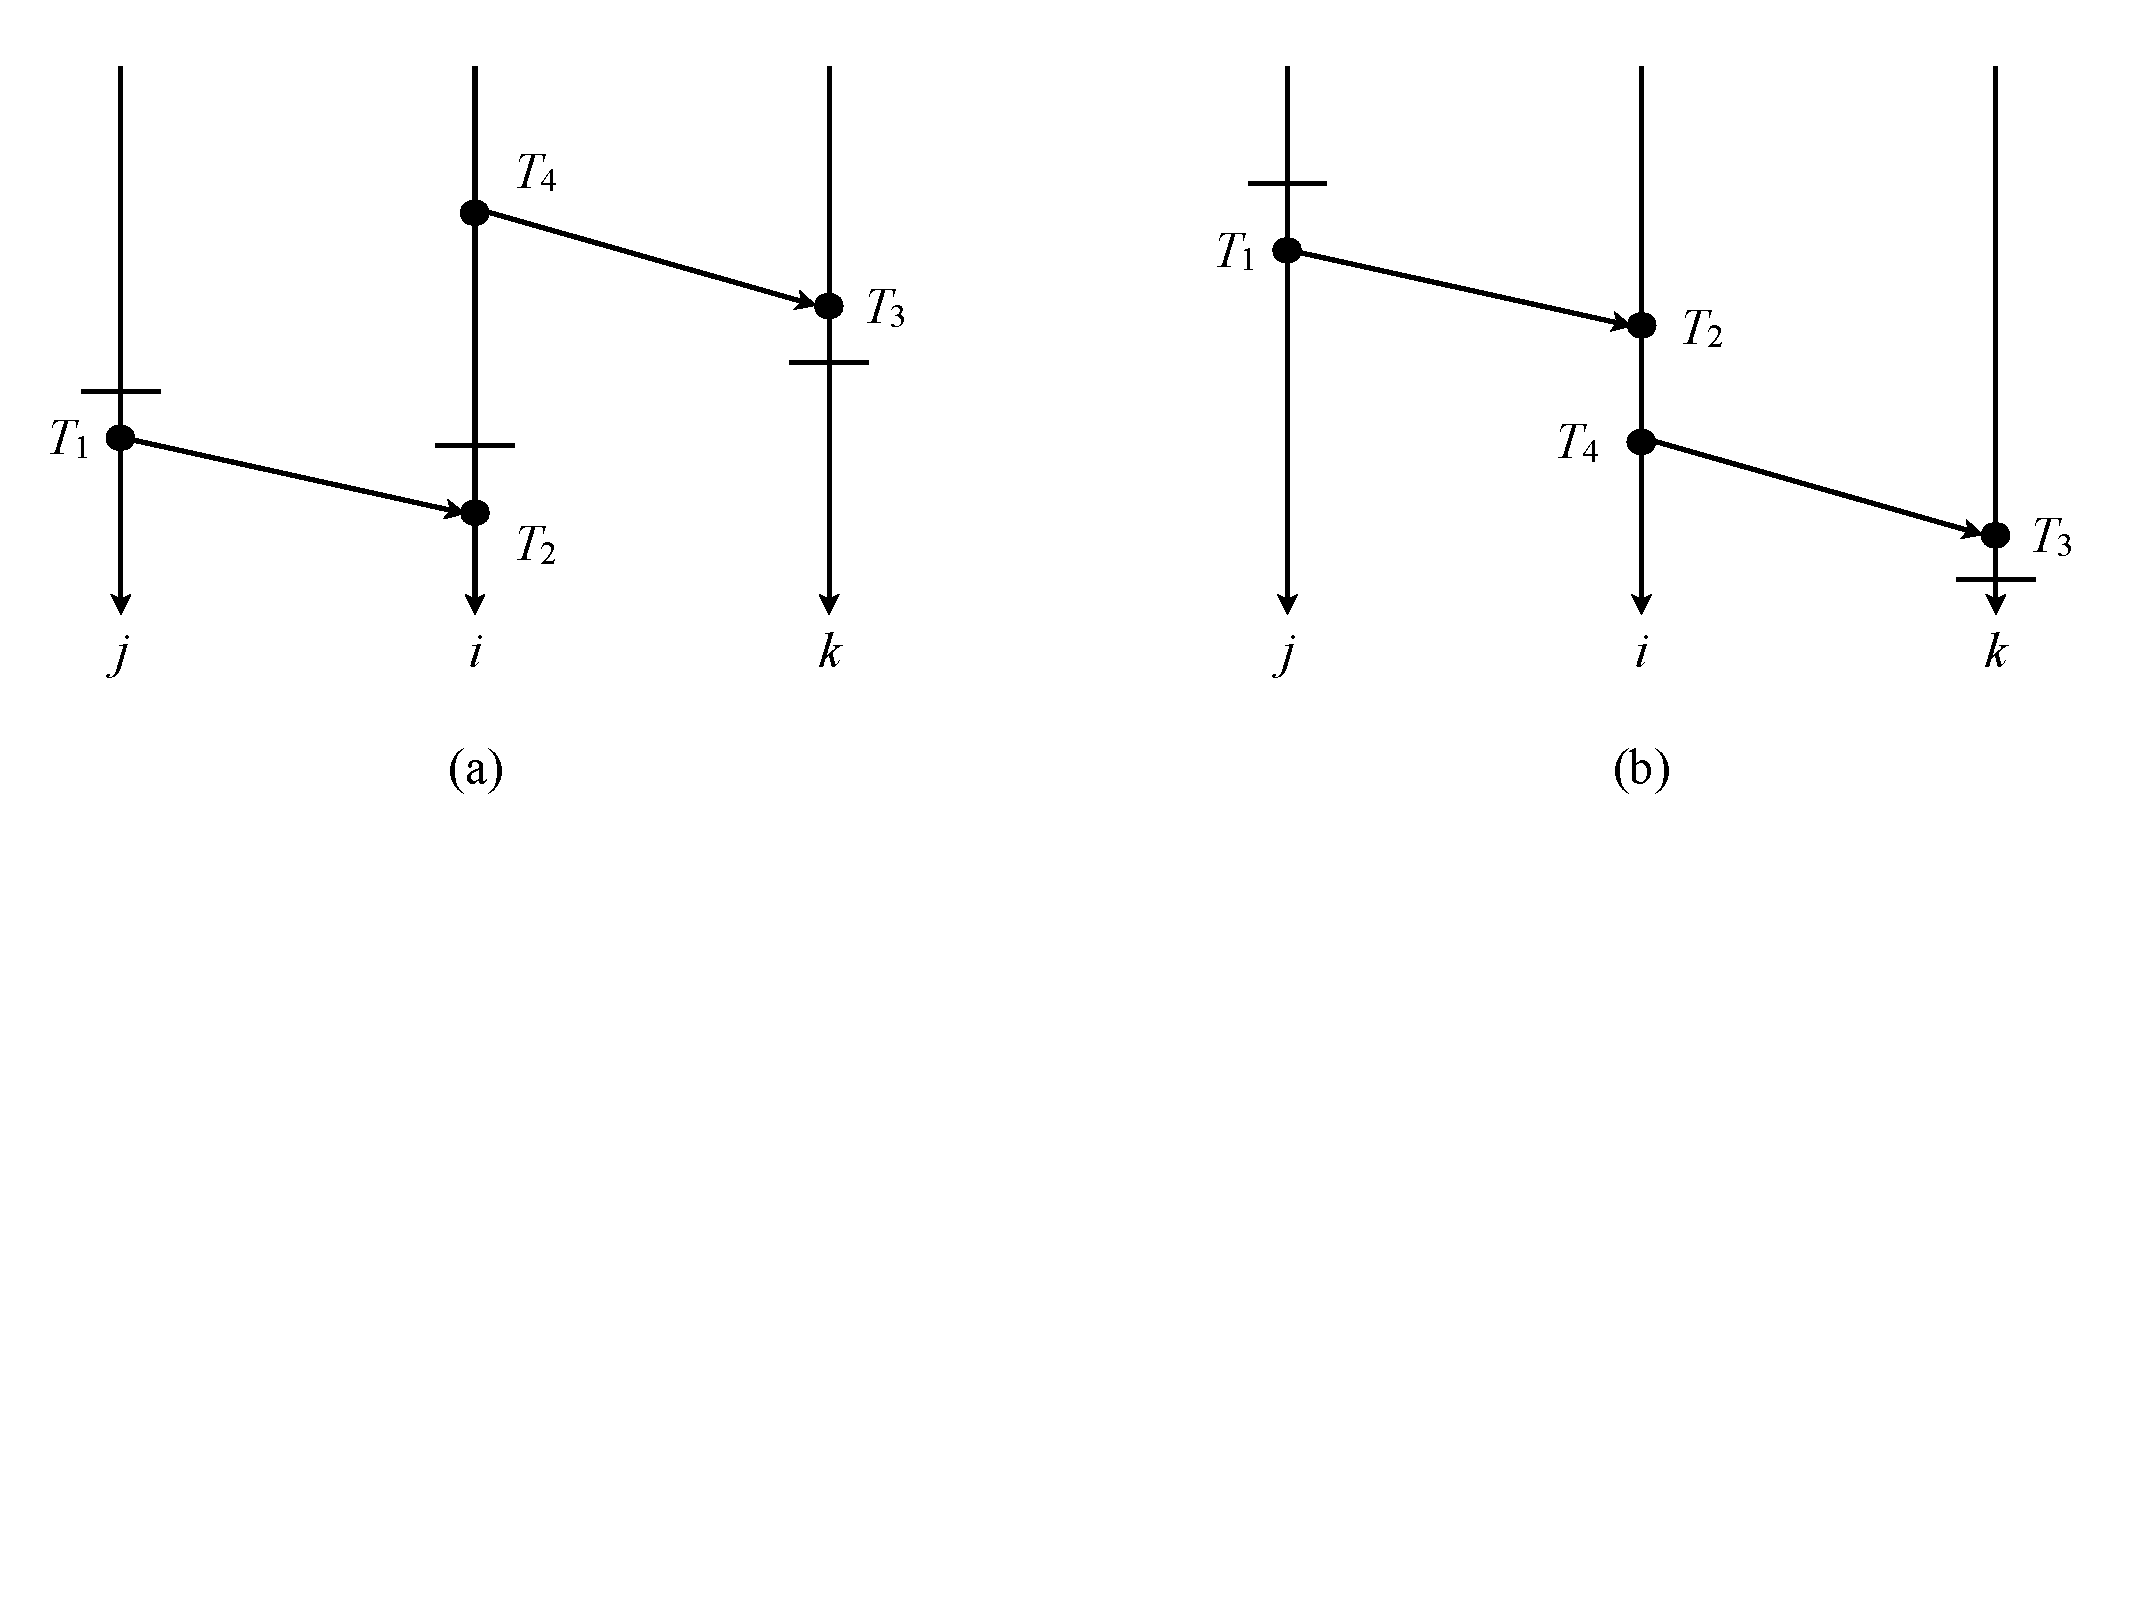
\includegraphics[width=\textwidth]{figures/ch4_snapshot.pdf}
\vspace{-6.5cm}
\caption{Illustrations of the snapshot computation. Vertical lines depict the
  commit order at the corresponding partitions (top to bottom) and horizontal
  lines the cut-offs of various snapshots. Arrows between partitions depict
  causal dependencies.}
\label{fig:snapshot}
\end{figure}

On the one hand, the snapshot cannot be too fresh. For example, suppose a transaction $\tx_1$ writing to some partition $j$ is excluded from the snapshot chosen by $\tx$ at $j$. Then, the snapshot chosen by $\tx$ at $i$ cannot contain $\tx_1$, nor any other transaction that causally depends on it, like $\tx_2$ (Figure~\ref{fig:snapshot}a). If the snapshot chosen by $\tx$ included $\tx_2$, it would be able to read some of $\tx_2$'s writes at $i$, thereby forcing $\tx$ to read the writes by $\tx_2$'s causal dependencies, including $\tx_1$; but $\tx$ cannot see these writes, because it excluded them from the snapshot at partition $j$. Thus, when building the snapshot, the server will need to take into account the snapshots taken by $\tx$ at the partitions it already read; the server selects the longest prefix of $\CommitLog$ transactions, such that their writes---and the ones by their causal dependencies---are included in $\tx$'s previous snapshots. This prefix is denoted by $r$ (line~\ref{alg:max_vc_search}), and is computed using the $\Vaggr$ vector included in each of the entries of $\CommitLog$, summarising the causal dependencies of all transactions up to a given record in the log. Thus, the snapshot at $s_i$ includes all transactions with sequence numbers up to $r.\Vaggr[i]$.

On the other hand, the snapshot selected cannot be too stale. Continuing with the previous example, if a transaction $\tx_3$ is included in the snapshot taken by $\tx$ at some partition $k$, then the snapshot of $\tx$ at partition $i$ has to include the writes by $\tx_3$ and its causal dependencies, e.g., the transaction $\tx_4$ in Figure~\ref{fig:snapshot}a. The writes of transactions---and of its causal dependencies---in the snapshots that $\tx$ has already fixed are summarised by $\VCaggr$. Thus, after determining the appropriate snapshot in line~\ref{alg:max_vc_search}, the server $s_i$ checks that this snapshot covers transactions with sequence numbers at $i$ up to $\VCaggr[i]$ (line~\ref{alg:read_req_abort_check}). To maximise the chances of passing this check, before allowing a transaction $\tx$ to proceed with a read, the server $s_i$ waits until the writes from the prefix up to $\VCaggr[i]$ have been incorporated into its state (line~\ref{alg:read_req_wait}).

It may be the case that it's impossible to satisfy both of the above requirements when selecting a snapshot; e.g., in the situation illustrated in figure~\ref{fig:snapshot}b. Assuming that the transaction $\tx$ has fixed a valid snapshot at $j$ and $k$, it is impossible to build a consistent snapshot at partition $i$; given that $\tx$ included $\tx_3$ at partition $k$, it is forced to read $\tx_4$'s writes at $i$. At the same time, because it excluded $\tx_1$ from the snapshot at $j$, $\tx$ can't read the writes by $\tx_2$ at $i$. In this case, without our second requirement, the server $s_i$ would build a snapshot excluding both $\tx_2$ and $\tx_4$, violating $T$'s causal dependency on $\tx_3$. In this case the server sends to the client a $\READRETURN$ message with a special value $\abort$ (line~\ref{alg:read_req_abort}), which will cause the client to abort the transaction (line~\ref{alg:read_abort}).

Once the server fixes a new snapshot, it selects the most recent version of the object $x$, defined by $e.\Vaggr[i]$ (line~\ref{alg:chose-version}), to return to the client. The server replies with a $\READRETURN$ message, carrying a triple of the value of the object, its associated version vector, and the aggregate vector for $e.\Vaggr$, summarising the causal dependencies of all the transactions in the snapshot. When the client receives the message (line~\ref{alg:read_msg_decomp}), it first sets the $j$-th entry of $\tx.\hasRead$ to $\top$, to indicate that $\tx$ has read an object at partition $j$, and joins the returned aggregate vector to $\tx.\VCaggr$. The client also joins the commit vector associated with the version read to a \emph{dependency vector} $\tx.\VCdep$, which represents all causal dependencies developed by $\tx$ during its execution. This ensures that, upon reading a version of object $x$, $\tx$ will causally depend on the transaction $\tx'$ that wrote that version of $x$, along with the causal dependencies of $\tx'$.

\subsection{Transaction Termination}

A client executing a transaction $\tx$ tries to commit it by calling a {\tt commit} function (line~\ref{alg:commit_start}). Read-only transactions are committed without any additional checks, since they already read a causally consistent snapshot (line~\ref{alg:commit_readonly_start}). To commit an update transaction $\tx$, we use a variant of the classical \emph{two-phase commit protocol (2PC)} among the processes that store the objects written by the transaction; the client executing $\tx$ servers as the 2PC coordinator.

In more detail, to commit a transaction $\tx$, the client first sends a $\PREPARE$ message to all servers storing the objects written by the transaction (line~\ref{alg:commit_send_loop}). The message contains $\tx$'s write-set and its dependency vector $\tx.\VCdep$. When a server $s_i$ receives this message (line~\ref{alg:prepare_start}), it \emph{validates} the transaction, deciding whether it can commit or abort due to conflicting concurrent transactions. The server then replies to the client with a \emph{vote} representing its decision. Based on the votes, the client determines the final decision on the transaction---the transaction commits if all votes are positive---and distributes the decision to the relevant servers.

\begin{figure}[htb!]
\begin{algorithm}[H]
  % Commit
  \SubAlgo{\Fun ${\tt commit}(T)$\label{alg:commit_start}}{
    \If{$\tx.\WS = \emptyset$\label{alg:commit_readonly_start}}{
      \Return{$\commit$}\;\label{alg:commit_readonly_end}
    }

    \ForAll{$\partj \in \partitions(\tx.\WS)$\label{alg:commit_send_loop}}{
      \Send{$\PREPARE(T, T.\WS, \VCdep)$} \KwTo $\partj$\;\label{alg:commit_send_prepare}
    }

    $\commitVC \leftarrow \tx.\VCdep$\; \label{alg:commit_commitvc_firstassignment}
    $\outcome \leftarrow \commit$\;

    \ForAll{$\partj \in \partitions(\tx.\WS)$\label{alg:commit_send_votes}}{
      \Receive{$\VOTE(m)$} \KwFrom $\partj$\;\label{alg:commit_recv_vote}
      \uIf{$m = \langle T, \abort \rangle$\label{alg:commit_vote_check}}{
        $\outcome \leftarrow \abort$\;
        \Break\;
      }
      \ElseIf{$m = \langle T, \commit, k \rangle$\label{alg:commit_vote_check_else}}{
        $\commitVC[j] \leftarrow k$\;\label{alg:commit_assign_seqn}
      }
    }

    \ForAll{$\partj \in \partitions(\tx.\WS)$}{
      \Send{$\DECIDE(\tx, \commitVC,\outcome)$} \KwTo $\partj$\;\label{alg:commit_send_decide}
    }

    \Return{$\outcome$}\;\label{alg:commit_end}
  }

  \smallskip

  % Prepare
  \SubAlgo{\WhenReceived $\PREPARE(\tx, \localWS, \localVdep)$ \KwFrom
    $c_j$\label{alg:prepare_start}}{
    \uIf{$(\exists T'.\
      (\langle T', \pending, \localWS' \rangle \in \cqueue \vee \langle T',
      \ready, \_, \_ \rangle \in \cqueue)
        \wedge{}$ $\localWS' \cap \localWS \ne
        \emptyset) \vee (\exists x.\, x \in \localWS \wedge
        \left(\VersionLog[x].\last.\Vcomm[i] > \localVdep[i]\right)$\label{alg:conflict_check}}{
      \Send{$\VOTE(t, \abort)$} \KwTo $c_j$\; \label{alg:send_abort}
    }\Else{
    $\lastprep \leftarrow \lastprep + 1$\;\label{alg:lastprep_incr}
    $\cqput(\tx, \pending, \localWS)$\;\label{alg:queue_put}
    \Send{$\VOTE(\tx, \commit, \lastprep)$} \KwTo $c_j$\;\label{alg:prepare_end}
  }}

  \smallskip

  % Decide
  \SubAlgo{\WhenReceived $\DECIDE(\tx, \commitVC, \mathit{decision})$ \KwFrom
    $\partj$\label{alg:decide_start}}{
    \uIf{$\mathit{decision} = \commit$\label{alg:decide_if}}{
      $\cqupdate(\langle \tx, \ready, \_, \commitVC\rangle)$\;\label{arg:queue_update}
    }
    \Else{
      $\cqremove(\tx)$\;\label{alg:decide_end}
    }
  }
\end{algorithm}
\caption{Commit protocol of a transaction and two-phase commit at server $s_i$}
\end{figure}

We now describe how a server $s_i$ computes its vote on a transaction (line~\ref{alg:conflict_check}). The vote for a transaction $\tx$ ensures the following property, used to validate the \Wconflict axiom of PSI: \todo{Reference back to the model in previous chapter}

\begin{itemize}
    \item \emph{For any pair of distinct transactions $\tx_1$ and $\tx_2$ writing to an object $x$, if $\tx_1$ precedes $\tx_2$ in the commit order, then $\tx_2$ will se the version of $x$ at least as up-to-date as the one written by $\tx_1$.}
\end{itemize}

To ensure this property, the server $s_i$ first check whether, for the objects that $\tx$ wrote to, the versions that $\tx$ read are still the most up-to-date ones in the database of $s_i$ at the time of validation. The server then checks whether $\tx$ conflicts with any transactions present in $\CommitQueue$, which have started committing at the server, but whose writes have not been applied to the database yet---the server aborts $\tx$ if any transaction $\tx'$ in $\CommitQueue$ writes to the same object as $\tx$. The writes in $\CommitQueue$ may be applied to the database before the writes of $\tx$, so checking for conflicts with them ensures that $\tx$'s reads will still be up-to-date when $\tx$'s writes are applied to the database.

If the validation for transaction $\tx$ fails, the server sends a $\VOTE$ message with the vote \abort, which tells the client to abort the transaction. If the validation succeeds, the server generates a sequence number for the transaction by incrementing $\lastprep$ and sends to the client a $\VOTE$ message with this sequence number and a vote \commit. The server also adds an entry $\langle \pending, \tx, \tx.\WS \rangle$ to the $\CommitQueue$, to record the fact that it is trying to commit $\tx$ at the server (lines~\ref{alg:lastprep_incr}--\ref{alg:prepare_end}).

The client waits until it receives $\VOTE$ messages from all involved servers (line~\ref{alg:commit_recv_vote}). If all the servers voted \commit, the client constructs the final commit vector for $\tx$ by changing its dependency vector $\tx.\VCdep$, so that it covers not only $\tx$'s causal dependencies, but also all its writes. These writes are identified by the sequence numbers provided by the servers as part of their $\VOTE$ messages. Thus, the commit vector is defined by setting the entries in $\tx.\VCdep$ for partitions written by $\tx$ to these sequence numbers (line~\ref{alg:commit_assign_seqn}). The client then sends a $\DECIDE$ message to all the involved servers with the final decision on $\tx$ along with its commit vector (line~\ref{alg:commit_send_decide}).

Upon receiving the decision on a transaction $\tx$ (line~\ref{alg:decide_start}), a server updates the entry associated with $\tx$ in $\CommitQueue$, to change its status to $\ready$ and record its commit vector. If the transaction is aborted, the server removes $\tx$ from the queue.

\begin{figure}[h]
\begin{algorithm}[H]
  % Queue head
  \SubAlgo{\Upon $\langle T, \ready, \localWS, \commitVC\rangle =
    \cqhead()$\label{alg:queue_start}}{
    $\cqremove(T)$\;\label{alg:queue_end}
    \ForAll{$\{\langle x , v \rangle \mid \langle x , v \rangle \in \localWS \wedge \partitionof(x) = i\}$} { \label{alg:queue_loopws}
        $\vlapply(\langle x , v , \commitVC \rangle)$\;\label{alg:queue_vapply}
    }

    $\mrvc \leftarrow \max(\mrvc,\commitVC)$\;\label{alg:queue_mrvc}
    $\cladd(T, \mrvc)$\;\label{alg:queue_clog_add}
  }
\end{algorithm}
\caption{Partition state update at server $s_i$ after a transaction commits}
\end{figure}

Committed transactions are applied to the database in their order in $\CommitQueue$, i.e., the commit order. When a $\ready$ transaction $\tx$ gets to the head of the queue (line~\ref{alg:queue_start}), the server dequeues it and adds its writes to $\VersionLog$, tagged with its commit vector. The server then joins $\tx$'s commit vector to $\LocalTime$, and adds the transaction to $\CommitLog$, along with $\LocalTime$ as its aggregate vector.
